\documentclass[10pt,a4paper]{article}
\usepackage[margin=1.7cm,top=1.5cm,bottom=1.6cm]{geometry}
\usepackage{fontspec}
\setmainfont{DejaVu Serif}[Scale=0.9]
\setsansfont{DejaVu Sans}[Scale=0.88]
\setmonofont{DejaVu Sans Mono}[Scale=0.8]
\usepackage{microtype,booktabs,tabularx,longtable,array,graphicx,xcolor,enumitem,tikz,caption,titlesec,ragged2e}
\usetikzlibrary{arrows.meta,decorations.pathreplacing,shapes.geometric,positioning}
\usepackage[hidelinks]{hyperref}
\setlist{nosep,leftmargin=1.2em}
\setlength{\parskip}{3pt}\setlength{\parindent}{0pt}
\titleformat{\section}{\sffamily\bfseries\large}{\thesection}{0.6em}{}
\titleformat{\subsection}{\sffamily\bfseries\normalsize}{\thesubsection}{0.5em}{}
\titlespacing*{\section}{0pt}{8pt}{3pt}\titlespacing*{\subsection}{0pt}{5pt}{2pt}
\captionsetup{font={small,sf},labelfont=bf,skip=2pt}
\newcolumntype{Y}{>{\RaggedRight\arraybackslash}X}
\newcommand{\adr}[1]{\textsf{ADR-#1}}
\newcommand{\code}[1]{\texttt{\small #1}}
\renewcommand{\arraystretch}{1.12}

\begin{document}
\begin{center}
{\sffamily\bfseries\Large Architecting an Agentic SDLC Workflow}\\[2pt]
{\sffamily Issue in, pull request out on a fork of tinydb\,---\,roll number 2023114007}\\[1pt]
{\small Repository: \url{https://github.com/Ekansh0301/tinydb} \quad Pinned upstream commit \code{edff96a}, prepared base \code{8a94233}}
\end{center}

\section{Architecture}
The workflow turns an issue into a tested and reviewed pull request through the six required stages. It is one deterministic orchestrator that drives three builder agents, plus a separate reviewer agent that has no write access. Figure~\ref{fig:comp} is the component view; Table~\ref{tab:stages} lists the agent, artifact and check of each stage; Figure~\ref{fig:seq} is one real run.

\begin{figure}[ht]\centering
\resizebox{\linewidth}{!}{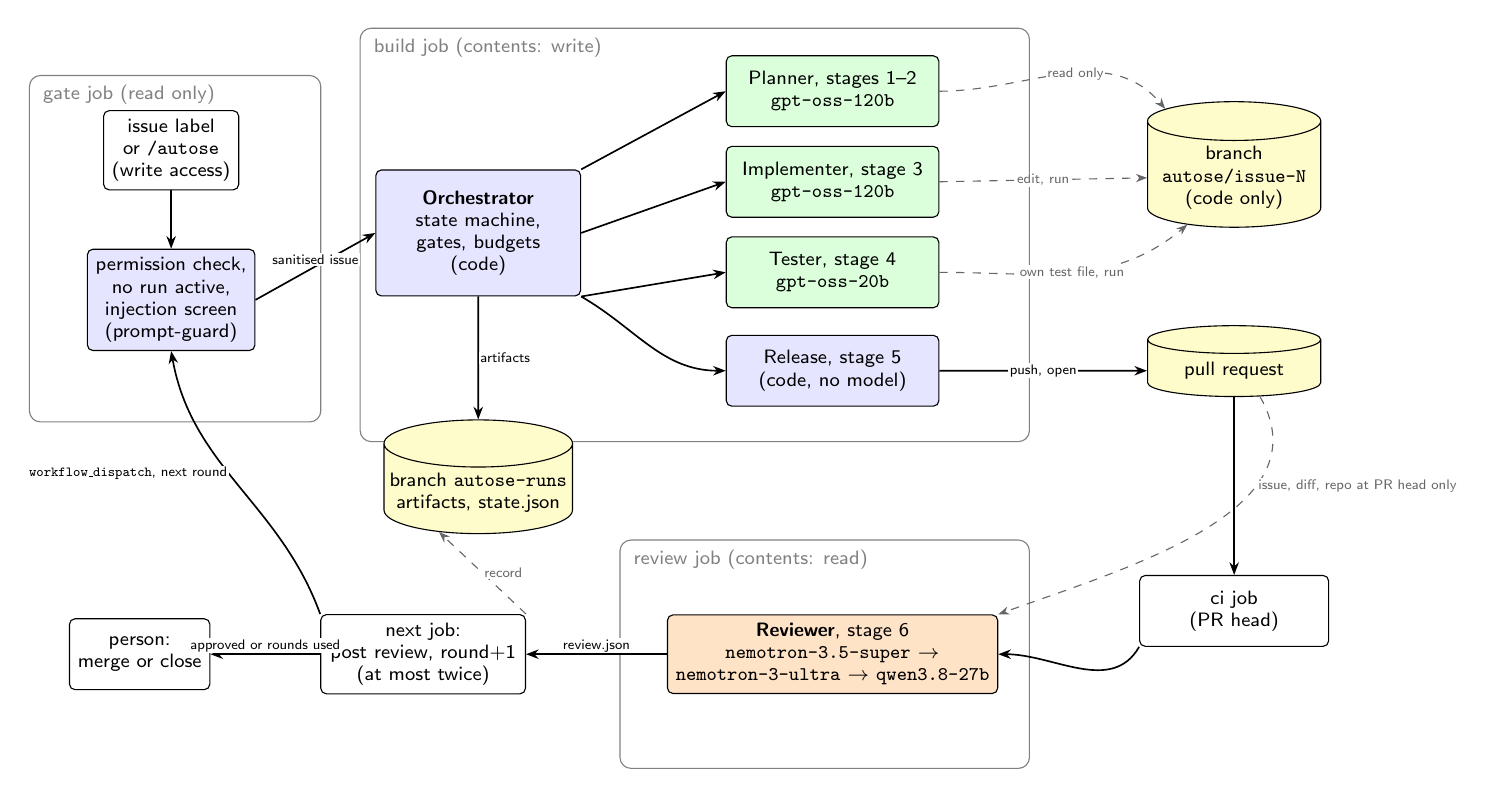
\begin{tikzpicture}[x=1cm,y=1cm,font=\sffamily\scriptsize,
  box/.style={draw,rounded corners=2pt,align=center,inner sep=3pt,minimum height=0.9cm},
  code/.style={box,fill=blue!10},
  agent/.style={box,fill=green!14,minimum width=2.7cm},
  rev/.style={box,fill=orange!22,minimum width=3.4cm},
  store/.style={draw,cylinder,shape border rotate=90,aspect=0.25,fill=yellow!20,align=center,inner sep=2pt,minimum height=0.9cm,minimum width=2.2cm},
  plain/.style={box,fill=white},
  a/.style={-{Stealth[length=1.6mm]},semithick},
  t/.style={-{Stealth[length=1.4mm]},dashed,gray!80!black},
  lab/.style={font=\sffamily\tiny,fill=white,inner sep=0.5pt}]
  % frames
  \draw[rounded corners=4pt,gray] (-0.2,-2.2) rectangle (3.5,2.2); \node[gray,anchor=north west] at (-0.15,2.2) {gate job (read only)};
  \draw[rounded corners=4pt,gray] (4.0,-2.45) rectangle (12.5,2.8); \node[gray,anchor=north west] at (4.05,2.8) {build job (contents: write)};
  \draw[rounded corners=4pt,gray] (7.3,-6.6) rectangle (12.5,-3.7); \node[gray,anchor=north west] at (7.35,-3.7) {review job (contents: read)};
  % top row
  \node[plain] (ev) at (1.6,1.25) {issue label\\ or \texttt{/autose}\\ (write access)};
  \node[code] (gate) at (1.6,-0.65) {permission check,\\ no run active,\\ injection screen\\ (prompt-guard)};
  \node[code,minimum width=2.6cm,minimum height=1.6cm] (orch) at (5.5,0.2) {\textbf{Orchestrator}\\ state machine,\\ gates, budgets\\ (code)};
  \node[agent] (plan) at (10.0,2.0) {Planner, stages 1--2\\ \texttt{gpt-oss-120b}};
  \node[agent] (impl) at (10.0,0.85) {Implementer, stage 3\\ \texttt{gpt-oss-120b}};
  \node[agent] (test) at (10.0,-0.3) {Tester, stage 4\\ \texttt{gpt-oss-20b}};
  \node[code,minimum width=2.7cm] (rel) at (10.0,-1.55) {Release, stage 5\\ (code, no model)};
  \node[store] (code) at (15.1,0.9) {branch\\ \texttt{autose/issue-N}\\ (code only)};
  \node[store] (runs) at (5.5,-3.1) {branch \texttt{autose-runs}\\ artifacts, state.json};
  \node[store] (pr) at (15.1,-1.55) {pull request};
  \node[plain,minimum width=2.4cm] (ci) at (15.1,-4.6) {ci job\\ (PR head)};
  \node[rev] (rev) at (10.0,-5.15) {\textbf{Reviewer}, stage 6\\ \texttt{nemotron-3.5-super} $\to$\\ \texttt{nemotron-3-ultra} $\to$ \texttt{qwen3.8-27b}};
  \node[plain,minimum width=2.6cm] (next) at (4.8,-5.15) {next job:\\ post review, round+1\\ (at most twice)};
  \node[plain] (human) at (1.2,-5.15) {person:\\ merge or close};
  % arrows
  \draw[a] (ev) -- (gate);
  \draw[a] (gate.east) -- node[lab,above] {sanitised issue} (orch.west);
  \draw[a] (orch.north east) -- (plan.west);
  \draw[a] (orch.east) -- (impl.west);
  \draw[a] (orch.south east) -- (test.west);
  \draw[a] (orch.south east) to[out=-30,in=180] (rel.west);
  \draw[t] (plan.east) to[out=0,in=130] node[lab,pos=0.55] {read only} (code.north west);
  \draw[t] (impl.east) -- node[lab] {edit, run} (code.west);
  \draw[t] (test.east) to[out=0,in=220] node[lab,pos=0.5] {own test file, run} (code.south west);
  \draw[a] (orch.south) -- node[lab,right] {artifacts} (runs.north);
  \draw[a] (rel.east) -- node[lab] {push, open} (pr.west);
  \draw[a] (pr.south) -- (ci.north);
  \draw[a] (ci.south west) to[out=-120,in=0] (rev.east);
  \draw[t] (pr.south east) to[out=-60,in=20] node[lab,pos=0.3,right] {issue, diff, repo at PR head only} (rev.north east);
  \draw[a] (rev.west) -- node[lab,above] {review.json} (next.east);
  \draw[a] (next.west) -- node[lab,above] {approved or rounds used} (human.east);
  \draw[a] (next.north west) to[out=110,in=-80] node[lab,left,pos=0.55] {\texttt{workflow\_dispatch}, next round} (gate.south);
  \draw[t] (next.north east) -- node[lab,right] {record} (runs.south west);
\end{tikzpicture}
}
\caption{Component view. Blue boxes are plain code, green boxes are builder agents, the orange box is the independent reviewer. Dashed arrows are tool access; every agent reaches the repository only through its own small tool set.}\label{fig:comp}
\end{figure}


\begin{table}[ht]\centering\small
\caption{Stage map: agent, artifact and check. A gate is decided by code (\adr{007}); an agent never says ``done''.}\label{tab:stages}
\begin{tabularx}{\linewidth}{@{}c l l l Y@{}}
\toprule
\# & Stage & Agent (model) & Artifact & Check before moving on \\ \midrule
1 & Requirements & Planner (\code{gpt-oss-120b}), A1 skill & \code{spec.md} & required sections; every criterion Given/When/Then with a concrete outcome; no vague word; each requirement has a criterion; one model call may only add ``not testable'' objections \\
2 & Design & Planner (same), A2 architecture note & \code{design.md} & every file and function named exists or is marked NEW; every criterion appears in a row \\
3 & Implementation & Implementer (\code{gpt-oss-120b}) & \code{diff.patch} & diff not empty; only files named in the design changed; compiles and imports \\
4 & Testing & Tester (\code{gpt-oss-20b}) & \code{test\_report.md} & a test \code{test\_ac<N>\_*} per criterion; at least one new test fails on the base commit; whole suite passes; fails go back to 3, a repeated failure to 1 \\
5 & Release & none (code) & \code{pr.md} + PR link & PR open; reusable CI workflow green on its head \\
6 & Review & Reviewer (Nemotron, separate job) & \code{review.md} & valid JSON with evidence for each check and a command run; approve, or two fix cycles used \\
\bottomrule\end{tabularx}
\end{table}


\begin{figure}[ht]\centering
\resizebox{\linewidth}{!}{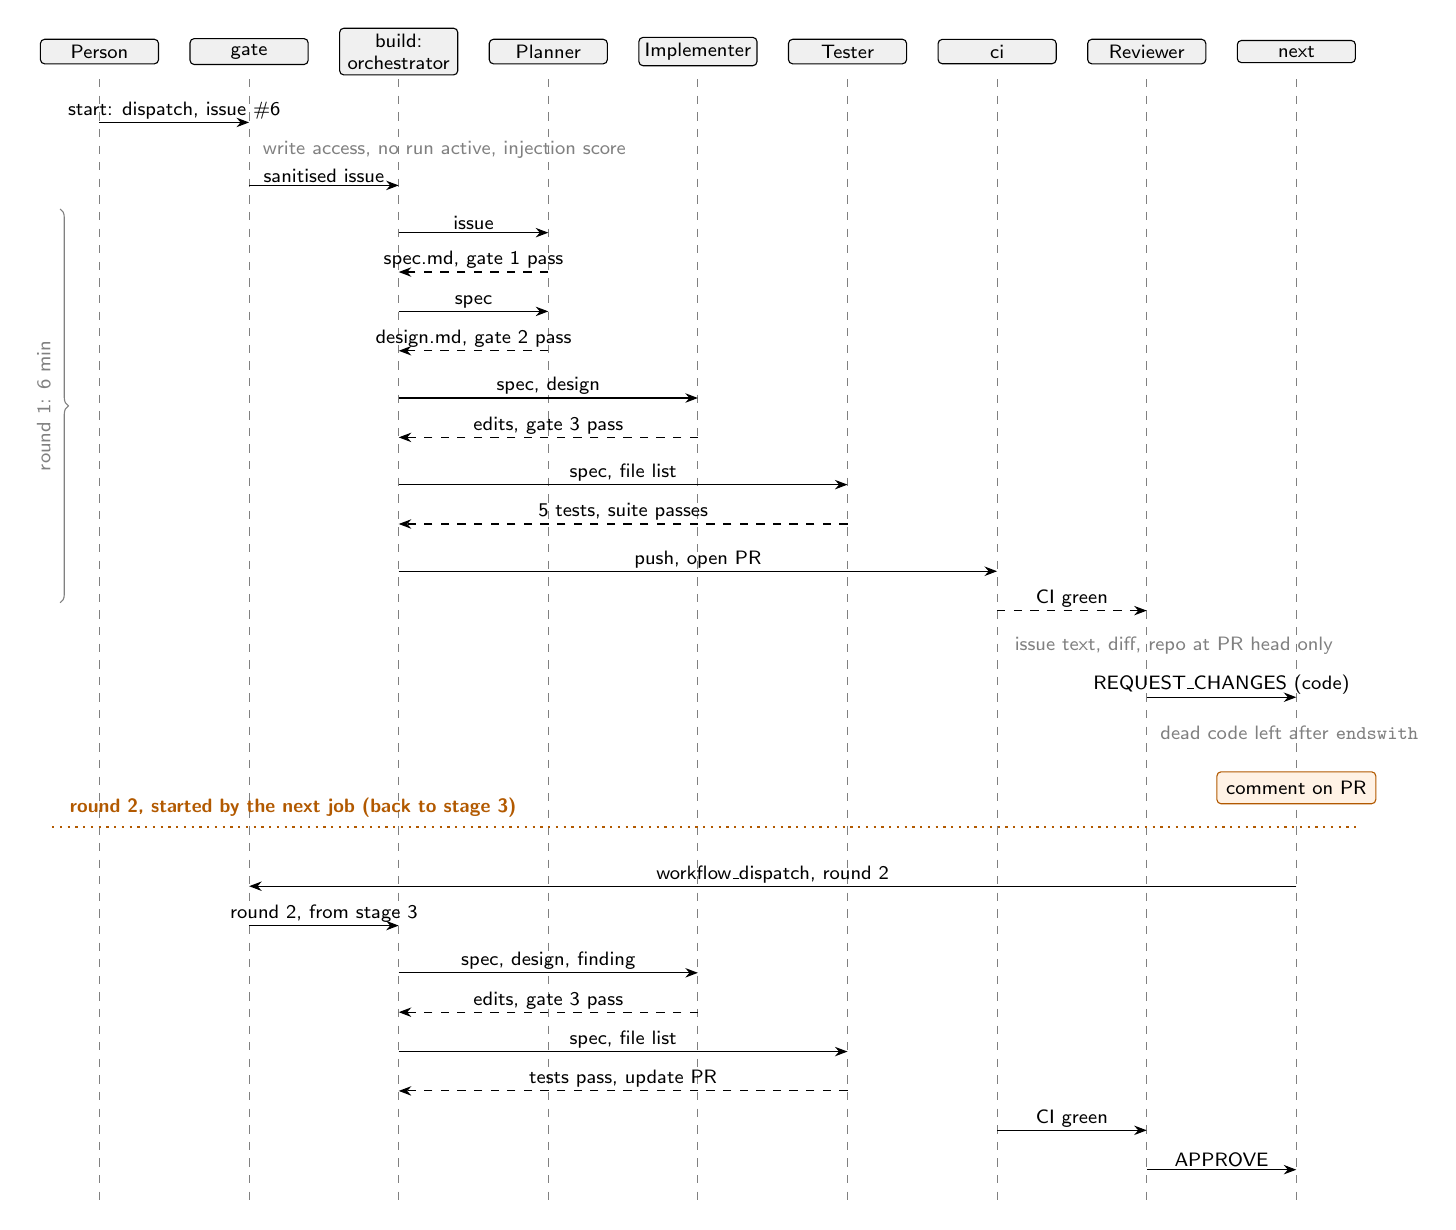
\begin{tikzpicture}[x=1cm,y=1cm,font=\sffamily\scriptsize]
  \def\top{0}\def\bot{-14.6}
  \foreach \x/\n in {0/Person,1.9/gate,3.8/{build:\\orchestrator},5.7/Planner,7.6/Implementer,9.5/Tester,11.4/{ci},13.3/Reviewer,15.2/next} {
    \node[draw,rounded corners=1.5pt,fill=gray!12,align=center,minimum width=1.5cm,inner sep=2pt] (n\x) at (\x,\top) {\n};
    \draw[dashed,gray] (\x,\top-0.35) -- (\x,\bot);
  }
  \tikzset{m/.style={-{Stealth[length=1.6mm]}},r/.style={-{Stealth[length=1.6mm]},dashed}}
  \newcommand{\msg}[4]{\draw[m] (#1,#3) -- node[above,pos=0.5,align=center,inner sep=1pt] {#4} (#2,#3);}
  \newcommand{\ret}[4]{\draw[r] (#1,#3) -- node[above,pos=0.5,align=center,inner sep=1pt] {#4} (#2,#3);}
  % ---- round 1 (run 44389251586)
  \msg{0}{1.9}{-0.9}{start: dispatch, issue \#6}
  \node[right,gray] at (1.95,-1.25) {write access, no run active, injection score};
  \msg{1.9}{3.8}{-1.7}{sanitised issue}
  \msg{3.8}{5.7}{-2.3}{issue}
  \ret{5.7}{3.8}{-2.8}{spec.md, gate 1 pass}
  \msg{3.8}{5.7}{-3.3}{spec}
  \ret{5.7}{3.8}{-3.8}{design.md, gate 2 pass}
  \msg{3.8}{7.6}{-4.4}{spec, design}
  \ret{7.6}{3.8}{-4.9}{edits, gate 3 pass}
  \msg{3.8}{9.5}{-5.5}{spec, file list}
  \ret{9.5}{3.8}{-6.0}{5 tests, suite passes}
  \msg{3.8}{11.4}{-6.6}{push, open PR}
  \ret{11.4}{13.3}{-7.1}{CI green}
  \node[right,gray,align=left] at (11.5,-7.55) {issue text, diff, repo at PR head only};
  \msg{13.3}{15.2}{-8.2}{REQUEST\_CHANGES (code)}
  \node[right,gray,align=left] at (13.35,-8.65) {dead code left after \texttt{endswith}};
  \node[draw=orange!70!black,fill=orange!10,rounded corners=1.5pt,font=\sffamily\scriptsize] at (15.2,-9.35) {comment on PR};
  % ---- round 2 (run 44390507790)
  \draw[dotted,orange!70!black,thick] (-0.6,-9.85) -- (16.0,-9.85);
  \node[orange!70!black,anchor=south west,font=\sffamily\scriptsize\bfseries] at (-0.5,-9.85) {round 2, started by the next job (back to stage 3)};
  \msg{15.2}{1.9}{-10.6}{workflow\_dispatch, round 2}
  \msg{1.9}{3.8}{-11.1}{round 2, from stage 3}
  \msg{3.8}{7.6}{-11.7}{spec, design, finding}
  \ret{7.6}{3.8}{-12.2}{edits, gate 3 pass}
  \msg{3.8}{9.5}{-12.7}{spec, file list}
  \ret{9.5}{3.8}{-13.2}{tests pass, update PR}
  \msg{11.4}{13.3}{-13.7}{CI green}
  \msg{13.3}{15.2}{-14.2}{APPROVE}
  \draw[decorate,decoration={brace,amplitude=3pt},gray] (-0.5,-2.0) -- (-0.5,-7.0) node[midway,left,rotate=90,anchor=south]{round 1: 6 min};
\end{tikzpicture}
}
\caption{One real run from the trigger to the review and the next round (Actions runs 44389251586 and 44390507790, issue \#6). All six stages passed in round 1 (6 minutes); the independent reviewer asked for a code change (dead code the tests cannot see) and the \code{next} job started round 2 at stage 3, after which the reviewer approved.}\label{fig:seq}
\end{figure}

\textbf{How the pieces fit.} The orchestrator (plain Python, \adr{002}) manages the state machine, the gates, and the budgets while the agents only make decisions on what to write or change during a stage. The agents transfer artifacts but never communicate with each other (\adr{003}, \adr{011}). The state exists on a different branch, \code{autose-runs}, and as workflow artifacts, with the pull request carrying only code (\adr{004}). The reviewer is a different job that has \code{contents: read}, a different family of models and its own prompt; its verdict leaves the job as a file and a later job posts it (\adr{008}). Anyone with write permission can start a run with a label or with the \code{/autose} comment, and the issue text is screened and passed to the agents as delimited data (\adr{009}, \adr{010}).

\section{Design decisions}
Table~\ref{tab:adr} summarises all twelve records. The full ADRs, including the evidence behind each amendment, are in \code{architecture/decisions/}; they follow the Nygard format used in the earlier study (status, context, decision, alternatives, consequences).

\begin{table}[ht]\centering\footnotesize
\caption{Summary of the decision records (all under \code{architecture/decisions/}).}\label{tab:adr}
\begin{tabularx}{\linewidth}{@{}l l Y Y Y l@{}}
\toprule
ADR & Area & Option chosen & Main option rejected & Main reason & Status \\ \midrule
001 & D1 Split & 3 builder agents + code release + separate reviewer & one agent for everything; one per stage & tester must not have seen the implementation; request limit forbids one long conversation & Accepted, tested (E1) \\
002 & D2 Control & deterministic state machine, bounded back-edges & planner agent decides what next & reproducible, auditable, budget-bounded & Accepted, 2 amendments \\
003 & D3 Hand-offs & short artifacts, never conversations & pass transcripts or summaries & limits error propagation and tokens & Superseded in part by 011 \\
004 & D4 State & files on branch \code{autose-runs} + artifacts + PR comment & artifacts in the PR branch; Actions cache & PR diff stays code only; durable and linkable & Accepted \\
005 & D5 Tools & in-process tools per role, empty command environment & MCP servers; \code{gh} for agents & least privilege; small tool list & Accepted (names changed) \\
006 & D6 Models & one pinned model per builder role; reviewer chain & cross-vendor fallback for builders & results attributable to one model; evidence from runs & Accepted, 5 amendments \\
007 & D7 Checks & code gates, model call may only object & LLM judge per stage & reproducible decisions & Accepted (gate bugs fixed) \\
008 & D8 Reviewer & own job, vendor, prompt, inputs, permissions + evidence rule & same model, fresh context & shared blind spots; rubber-stamping & Accepted, tested (E2) \\
009 & D9 Safety & budgets, delimiters, injection classifier, keyless commands & trust the model to ignore injections & defence in layers, measurable & Accepted \\
010 & D10 Triggers & label or \code{/autose} by write access; one run per issue & trigger on every issue & only maintainers spend tokens & Accepted, 1 amendment \\
011 & D3 Hand-offs & trimmed architecture note, small file reads & full note, free-size reads & first run exceeded the request limit & Accepted, supersedes 003 row \\
\bottomrule\end{tabularx}
\end{table}

\subsection*{The three decisions that mattered most}
\textbf{\adr{008}, reviewer independence.} Reviewers who have information about the builder's context tend to approve. The opposite can also happen: in one of the early tests, a model rejected even a harmless change. We therefore ensured independence at five levels (a separate job, a different model and vendor, its own prompt, its own inputs, and a command environment without keys) and added an evidence rule: a verdict is valid only if it has at least two checks with evidence and the reviewer ran a command. This rule proved useful on two occasions. In pull request \#34 the reviewer found a real defect (the query cache returns before the limit is applied) by running its own snippet, which is exactly what two hidden tests check. And reviews that came back as general comments, or that ran out of budget, were counted as no review and not as approval. The downside is that the reviewer saw neither the specification nor the design, so it judged the change on the issue text alone, which sometimes made it miss defects that only the specification would reveal (Section~\ref{sec:exp}).

\textbf{\adr{002}, a deterministic orchestrator with bounded back-edges.} If an agent decided when to go back, a faulty agent could bypass a gate or loop on a budget we cannot afford. The state machine kept every run on its designed path, with each stage doing only its own job, and it made errors visible, because every attempt of every stage is recorded in \code{stages.jsonl}. Real runs changed it twice (the amendments in \adr{002}): a criterion that fails twice now goes back to \emph{requirements}, because a repeated failure can come from a criterion that asks for something the code cannot provide, and tests that cannot even be collected are blamed on the tester, not on the implementer.

\textbf{\adr{006}, models chosen by measurement.} The free models limited everything. We first measured availability and tool-call behaviour, and then had to revise the choice five times because the runs contradicted the probes (probes from a laptop showed neither the quota, nor the hang, nor the truncated tool arguments that the runner showed). The main conclusion recorded in the ADR is that a model is chosen only after it has completed a stage inside the real workflow, and that each builder role is pinned to one model, so that results can be attributed to it (for this reason the fallback added by the second amendment was reverted).

\section{Decision experiments}\label{sec:exp}
The single-agent variant has no recorded runs yet.

\begin{table}[ht]\centering\small
\caption{E2, reviewer independence: all reviews by the final reviewer on the five seeded pull requests (three trials per pull request).}\label{tab:e2}
\begin{tabular}{@{}l r r r r r r r@{}}
\toprule
Variant & Reviews & Valid & Wrong PRs caught & Wrong PRs missed & Correct PRs approved & Correct PRs rejected & Mean tokens \\ \midrule
independent & 15 & 14 & 8/9 & 0/9 & 6/6 & 0/6 & 54124 \\
\bottomrule\end{tabular}
\end{table}
Pending.


\section{Results}\label{sec:results}
\begin{table}[ht]\centering\small
\caption{Per-stage pass rates over all recorded stage attempts (every run, including runs that later stopped).}\label{tab:rates}
\begin{tabular}{@{}l c r r r r@{}}
\toprule
Variant & Stage & Attempts & Passed & Rate & First-attempt rate \\ \midrule
pipeline & 1 & 14 & 11 & 79\% & 82\% \\
pipeline & 2 & 17 & 9 & 53\% & 50\% \\
pipeline & 3 & 19 & 15 & 79\% & 82\% \\
pipeline & 4 & 20 & 5 & 25\% & 40\% \\
single & single & 3 & 0 & 0\% & 0\% \\
\bottomrule\end{tabular}
\end{table}
\begin{table}[ht]\centering\small
\caption{Result of each pipeline or variant round: hidden acceptance tests (passed/total), regressions among the 228 baseline tests, and the reviewer's verdict on that round.}\label{tab:issues}
\begin{tabular}{@{}r l c c c c r r l@{}}
\toprule
Issue & Variant & Round & PR & Hidden & Regr. & Tokens & Reviewer & \\ \midrule
\#4 & pipeline & 1 & \#48 & not scored & -- & 160447 & approve & \\
\#5 & pipeline & 1 & -- & not scored & -- & 227977 & none & \\
\#6 & pipeline & 1 & \#49 & not scored & -- & 120598 & request changes & \\
\#6 & pipeline & 2 & \#49 & not scored & -- & 19735 & approve & \\
\#7 & pipeline & 1 & \#34 & 3/5 & 0 & 215385 & request changes & \\
\#7 & pipeline & 2 & \#34 & not scored & -- & 23821 & approve & \\
\#8 & pipeline & 1 & -- & not scored & -- & 195881 & none & \\
\#4 & single & 1 & -- & not scored & -- & 129210 & none & \\
\bottomrule\end{tabular}
\end{table}
\begin{table}[ht]\centering\small
\caption{Reviewer calibration on the five seeded pull requests: outcome of every trial. A correct pull request should be approved; a wrong one should be rejected.}\label{tab:seeded}
\begin{tabular}{@{}l l l l@{}}
\toprule
Variant & PR (label) & Outcomes by trial & Right/valid \\ \midrule
independent v1 & \#13 (correct) & approved, no valid review, approved & 2/2 \\
independent v1 & \#14 (wrong) & caught, caught, caught & 3/3 \\
independent v1 & \#15 (correct) & approved, approved, approved & 3/3 \\
independent v1 & \#16 (wrong) & missed, missed, no valid review & 0/2 \\
independent v1 & \#17 (wrong) & caught, caught, caught & 3/3 \\
independent v2 & \#13 (correct) & approved, approved, approved & 3/3 \\
independent v2 & \#14 (wrong) & no valid review, caught, caught & 2/2 \\
independent v2 & \#15 (correct) & approved, approved, approved & 3/3 \\
independent v2 & \#16 (wrong) & missed, caught, caught & 2/3 \\
independent v2 & \#17 (wrong) & caught, no valid review, no valid review & 1/1 \\
independent v3 & \#13 (correct) & approved, approved, approved & 3/3 \\
independent v3 & \#14 (wrong) & no valid review, caught, caught & 2/2 \\
independent v3 & \#15 (correct) & approved, approved, approved & 3/3 \\
independent v3 & \#16 (wrong) & caught, caught, caught & 3/3 \\
independent v3 & \#17 (wrong) & caught, caught, caught & 3/3 \\
same-model v3 & \#13 (correct) & approved, approved, approved & 3/3 \\
same-model v3 & \#14 (wrong) & missed, missed, missed & 0/3 \\
same-model v3 & \#15 (correct) & no valid review, approved, approved & 2/2 \\
same-model v3 & \#16 (wrong) & missed, missed, missed & 0/3 \\
same-model v3 & \#17 (wrong) & missed, caught, missed & 1/3 \\
\bottomrule\end{tabular}
\end{table}


\section{Hindsight}
First of all, I would change \adr{006} and the way I used it. I chose models from probes run on my laptop with a few short requests, and then revised the choice five times because the real activity on the runner was different: Groq has a daily token quota, one endpoint hung only inside the pipeline, one model cut off the arguments of its own tool calls, and another got stuck exploring. Each revision cost me a run and about half a day. If I could restart, I would choose each model by running one complete stage on recorded data on a GitHub runner, work out the token budget first (about 150\,000 tokens per run against 1.2\,million per day), and pin one model per builder role from the start. Secondly, I would write gate unit tests from recorded agent output on day one, because four of the early stops were bugs in my gates (a hyphen, a table cell, a criterion that covers two requirements, and a function name with a comment) rather than mistakes of the agents.


\section{Limitations and threats to validity}
\begin{enumerate}
\item \textbf{Free hosted models that change under us.} All models are free preview endpoints with daily token quotas and some latency. Runs were spread over several days, the model choice was revised five times (\adr{006}), and no sampling seed was set. The builders are small models, so the numbers say little about frontier models, and a rerun on another day can give different results.
\item \textbf{The workflow was developed on the evaluation issue.} Gates, prompts and routing rules were tuned during the runs on issue \#7 (and on the artifacts of those runs). Results for that issue are therefore not blind, while the other issues are the fairer test. All failed attempts are kept and listed in \code{results/runs.md}.
\item \textbf{Hidden tests encode our reading of the issues.} Issue \#8 is vague, and its tests accept both readings (reject the combination, or restrict it to the intersection). The natural fix for issue \#5 conflicts with an existing test that locks in the old behaviour. A different, reasonable fix can fail a test, and a test can pass for the wrong reason.
\item \textbf{Incomplete token accounting.} Per-call token logging was added only after the first runs, and local development runs are not counted, so the total in the appendix is a lower bound.
\item \textbf{Reviewer independence is partial.} The reviewer is from a different vendor than the builders, but its first two tiers are both NVIDIA models, its third tier is a model that was also tried as tester, and all builders are from one family. If a reviewer fails (a prose answer, no evidence, or the budget used up), it is recorded as \emph{no review}, which is safe but lowers its measured catch rate.
\item \textbf{The injection defence is only partly measured.} The classifier misses polite instructions; the other layers held in one end-to-end test with one model, which is evidence, not proof. The screen was not working in the recorded runs until it was fixed (\adr{009}); the five issue texts are benign, so no result changes.
\item \textbf{Very small sample, no statistics.} Five issues in one repository, mostly one run per cell, and five seeded pull requests with two or three trials each. Differences between variants are described, not tested, and a single lucky or unlucky run can change a cell. The same person wrote the issues, the hidden tests, the seeded defects and the workflow.
\item \textbf{The planner sees a trimmed architecture note} (\adr{011}); we did not test whether the full note would have produced better designs.
\end{enumerate}


\appendix
\section{Appendix: runs, tokens and reproduction}
\textbf{Runs.} \code{results/runs.md} lists every Actions run with a note: 39 pipeline runs (21 were development attempts on issue \#7 before the freeze, which stopped for reasons recorded in the ADRs; the recorded baseline and experiment runs follow), 75 reviewer-calibration runs, and the probe run.

\textbf{Tokens.} Recorded in the logs of the Actions runs (every model call logs its token use): 8,475,322 tokens in total. The four rehearsal runs on \code{gpt-oss-20b} alone used 0.93\,M tokens (\code{experiment/rehearsal.md}); they, the earlier local development runs and the first runs, which did not yet log per call, are not included, so this is a lower bound. All models are free tiers, so the spending limit is zero.

By model: \code{groq:openai/gpt-oss-120b} 2,800,578; \code{nvidia:nvidia/nemotron-3.5-super-vl-120b-a12b} 2,688,505; \code{nvidia:nvidia/nemotron-3-ultra-550b-a55b} 1,778,623; \code{nvidia:poolside/laguna-xs-2.1} 678,263; \code{groq:qwen/qwen3.8-27b} 402,076; \code{groq:openai/gpt-oss-20b} 127,277; \code{groq:meta-llama/llama-prompt-guard-2-86m} 0.

\textbf{Reproduction.} \code{experiment/drive.py <issue> [--variant single]} starts a recorded run; \code{experiment/score.py} scores a pull request against the hidden tests (\code{experiment/hidden\_tests/}, added after the last run); \code{experiment/collect.py}, \code{experiment/tokens.py} and \code{report/build.py} rebuild the tables and this report. The frozen code is the tag \code{autose-v1} (crash fix \code{v1.1}; reviewer order \code{v1.2}, after the recorded runs).
\end{document}
